\Transcb{yellow}{blue}{Cosmic rays}
\begin{center}
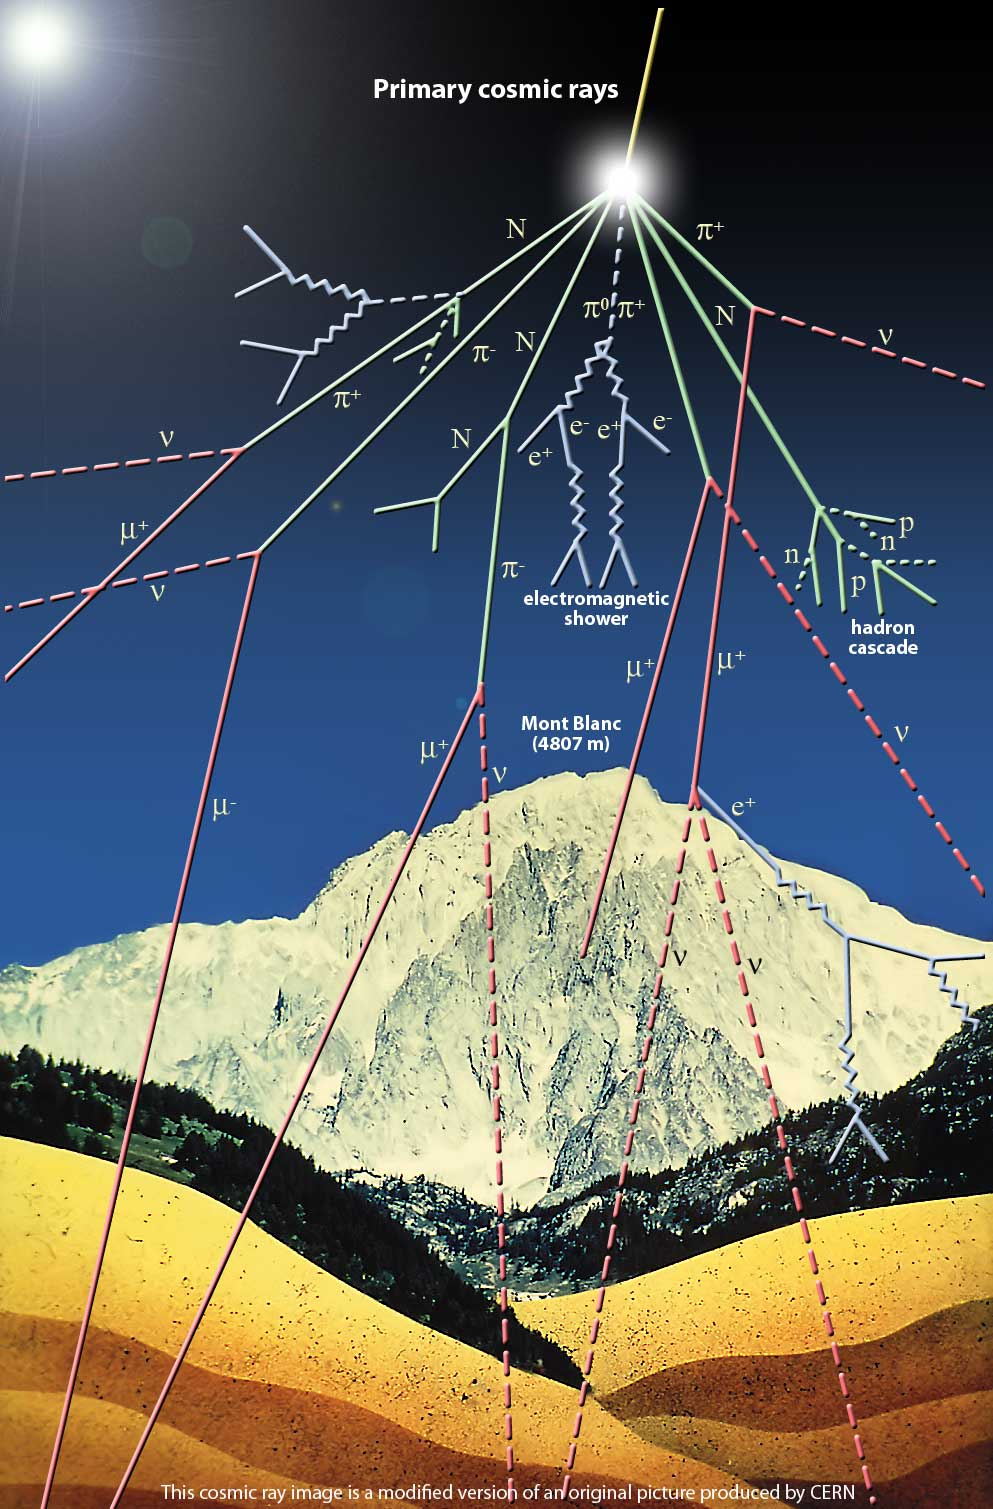
\includegraphics[keepaspectratio,height=15cm]{cosray}
\end{center}

\newpage

\vspace*{1cm}
\begin{itemize}
\item Observations :
\item[] Charge leaks slowly from capacitors
\item[] Effect is smaller when shielded
\item Idea :
\item[] Air gets ionised by charged particles
\item Where do these particles come from ?
\item[] From outer space (Hess 1912)
\item What sort of particles are these ?
\item[] Cosmic ray experiments
\end{itemize}

\Tr
\begin{center}
{\blue Cosmic ray spectra}\\[5mm]
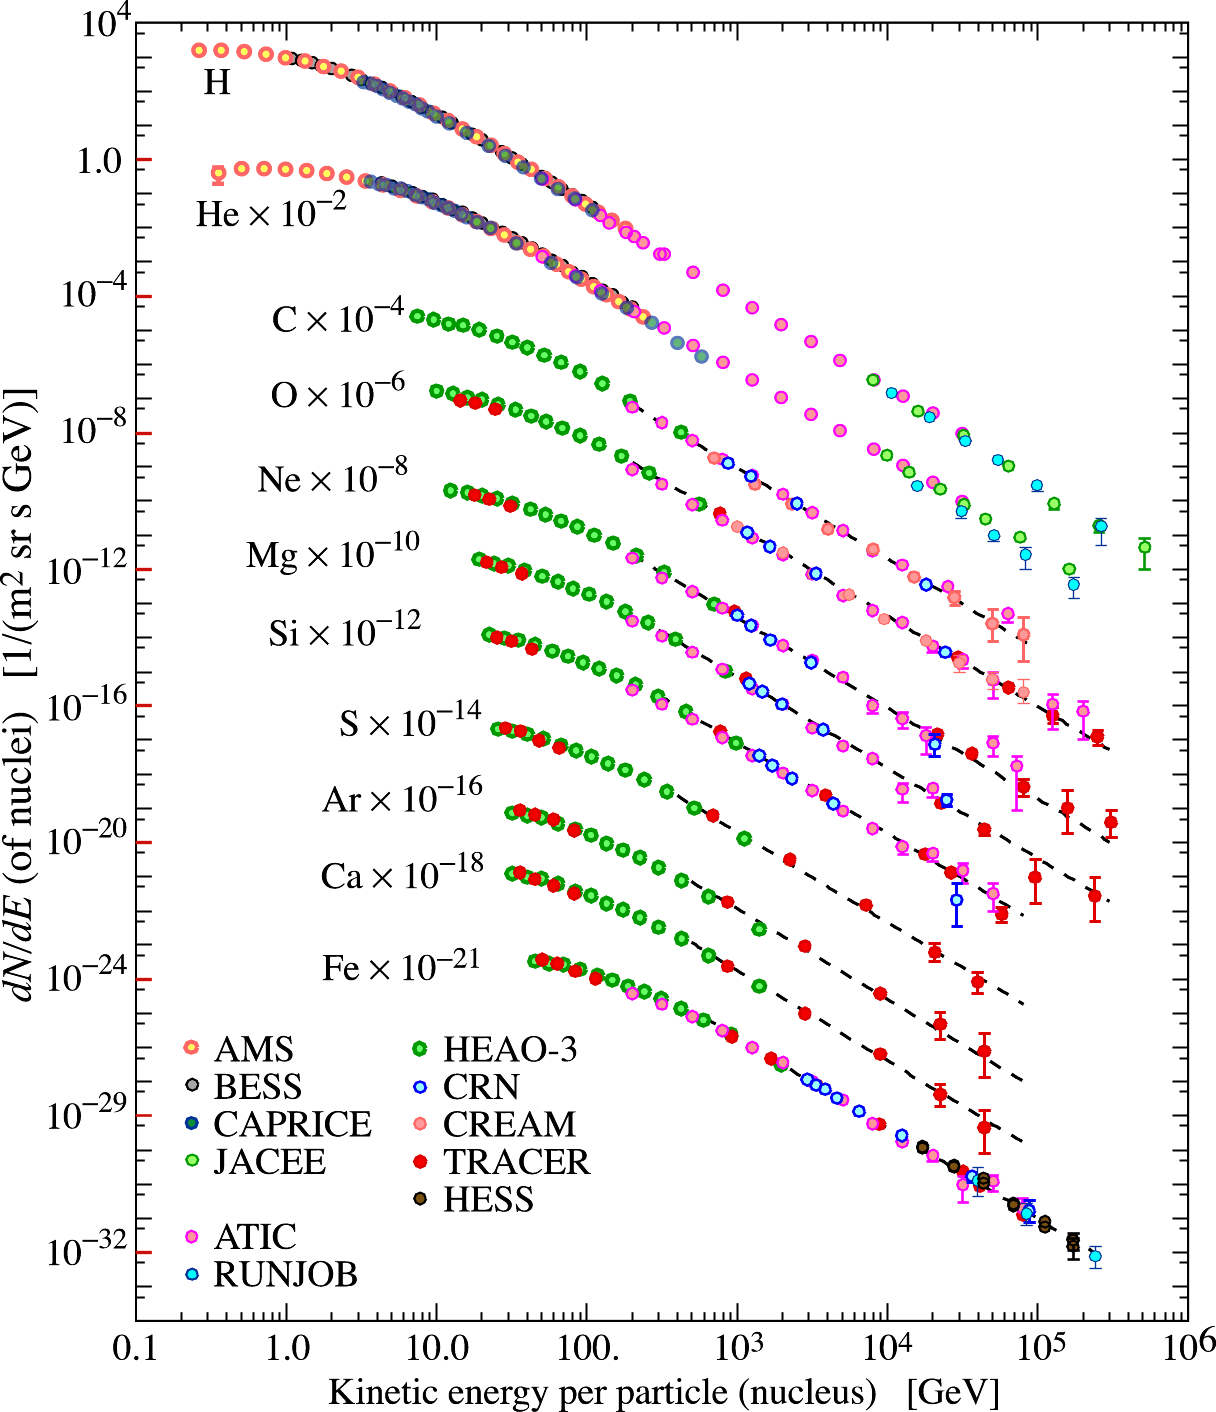
\includegraphics[keepaspectratio,height=14cm]{cr-low-e}
\end{center}

\newpage

\vspace*{1mm}
\begin{itemize}
\item[] Below 1 GeV $\rightarrow$ Solar modulation
\item[] At higher energies we observe
\item Proportions of major components\\
      relatively constant with energy
\item $\frac{\d N}{\d E} \propto E^{-2.7}$
\item Boron spectrum falls steeper
\item[] B is a spallation product of C and O
\item[] Secondary (e.g. spallation) nuclei steeper than primaries
\item sec./prim. decreases as energy increases
\item[] $\rightarrow$ High E rays diffuse out of galaxy faster
\end{itemize}
%
\colorbox{yellow}{What is the maximum energy~?}

\Tr
\vspace*{1.5cm}
\begin{center}
{\blue $E^{2.7}$ scaled flux}\\[5mm]
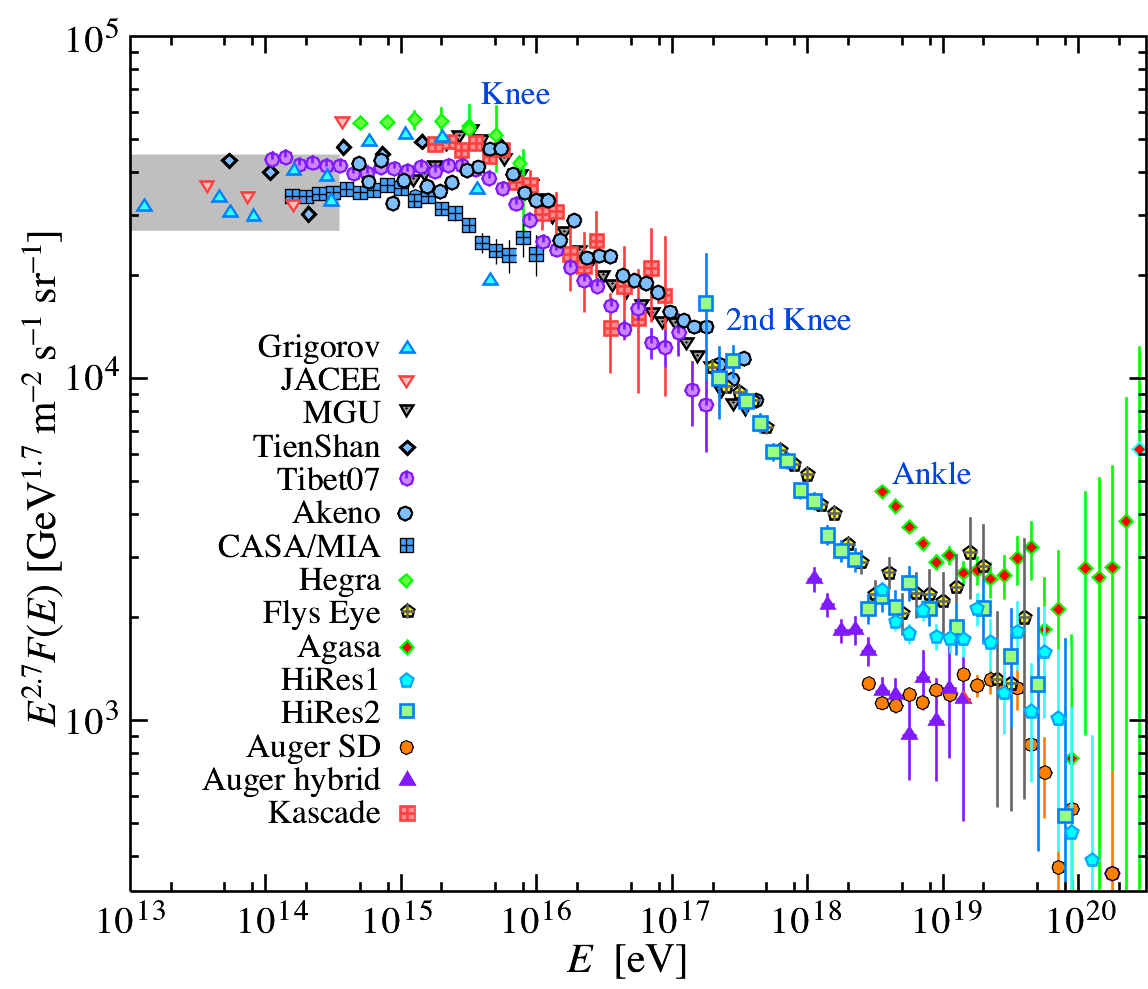
\includegraphics[keepaspectratio,width=12cm]{cr-all-scaled27}
\end{center}

\newpage

\vspace*{3cm}
\begin{itemize}
\item Spectral features observed (knee, ankle)
\item[] $E$ limits of different cosmic accelerators~?
\item[] What are these cosmic accelerator sites~?
\item Rather large uncertainties in flux 
\item[] Due to different exp. and models\\
        (see later)
\end{itemize}
%
\colorbox{yellow}{What is the cosmic acceleration mechanism~?}

\Tr
\twocolumn[\begin{center}{\blue Shock wave acceleration}\end{center}]
%
\begin{itemize}
\item Shock front due to an explosive event
\item[] Thin matter sheet with $v>v_{sound}$
\item[] $\rightarrow$ bulk motion ($\Delta v$) after the shock
\item Let a particle enter downstream of the shock
      and pass the front
\item[] {\blue Energy gain $\Delta E=\alpha E \quad (\alpha \propto \Delta v/c)$}
\item[] May backscatter downstream again
\item[] $\rightarrow$ process may be repeated
\item {\blue Multy-step particle acceleration}
\item[] Start energy $E_{0}$ and escape prob. $P_{esc}$
\item[$\ast$] After $n$ encounters~: $E_{n}=E_{0}(1+\alpha)^{n}$
\item[] $\rightarrow n=\frac{\ln(E/E_{0})}{\ln(1+\alpha)}$ to reach energy $E$
\item[] and $P_{stay}(n)=P_{stay}^{n}=(1-P_{esc})^{n}$
\end{itemize}

\newpage

\begin{itemize}
\item Number of particles with energy above $E$
\item[] $\displaystyle N(>E) \propto \sum_{k=n}^{\infty} P_{stay}^{k}
        =\frac{\left(1-P_{esc}\right)^{n}}{P_{esc}}$
\item[] Resulting in a spectrum
\item[] \begin{center}
        {\blue $N(>E) \propto \frac{1}{P_{esc}} \left(\frac{E}{E_{0}}\right)^{-\beta}$}
        \end{center}
\item[] where $\beta=\frac{-\ln(1-P_{esc})}{\ln(1+\alpha)} \approx \frac{P_{esc}}{\alpha}$
\end{itemize}

\begin{center}
\colorbox{yellow}{Indeed a powerlaw spectrum is obtained !}
\end{center}

\begin{itemize}
\item[] Note~: $P_{esc}$ is related to mean free path
\item[] \colorbox{yellow}{Spectral slope $\beta \propto (\sigma \cdot \text{density})^{-1}$}
\item[] {\blue Where do we find shock waves ?}
\end{itemize}

\Tr
\onecolumn
\begin{center}
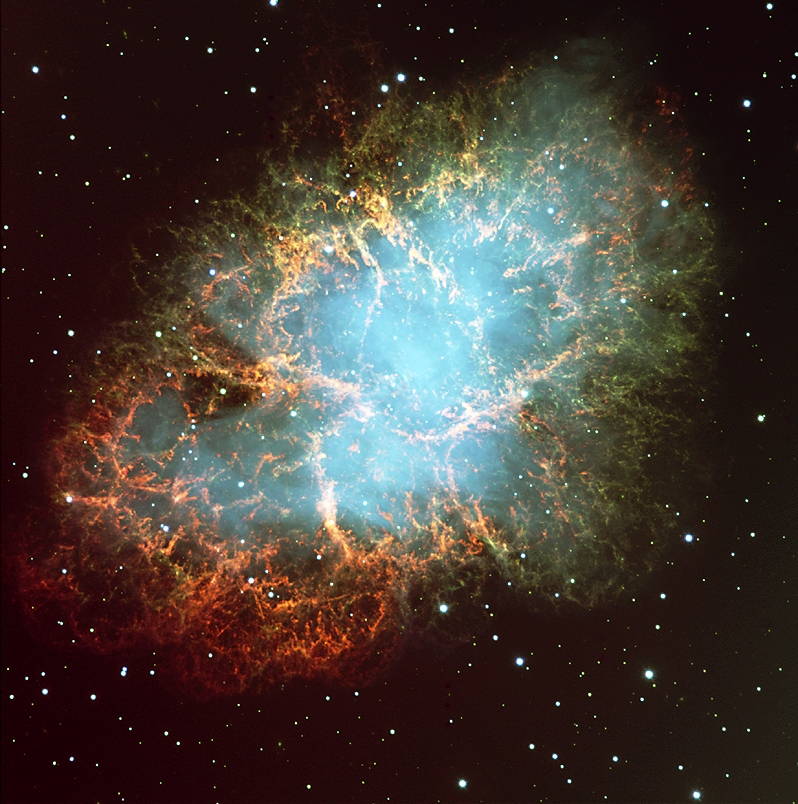
\includegraphics[keepaspectratio,height=15cm]{crab}
\end{center}

\Tr
\begin{center}
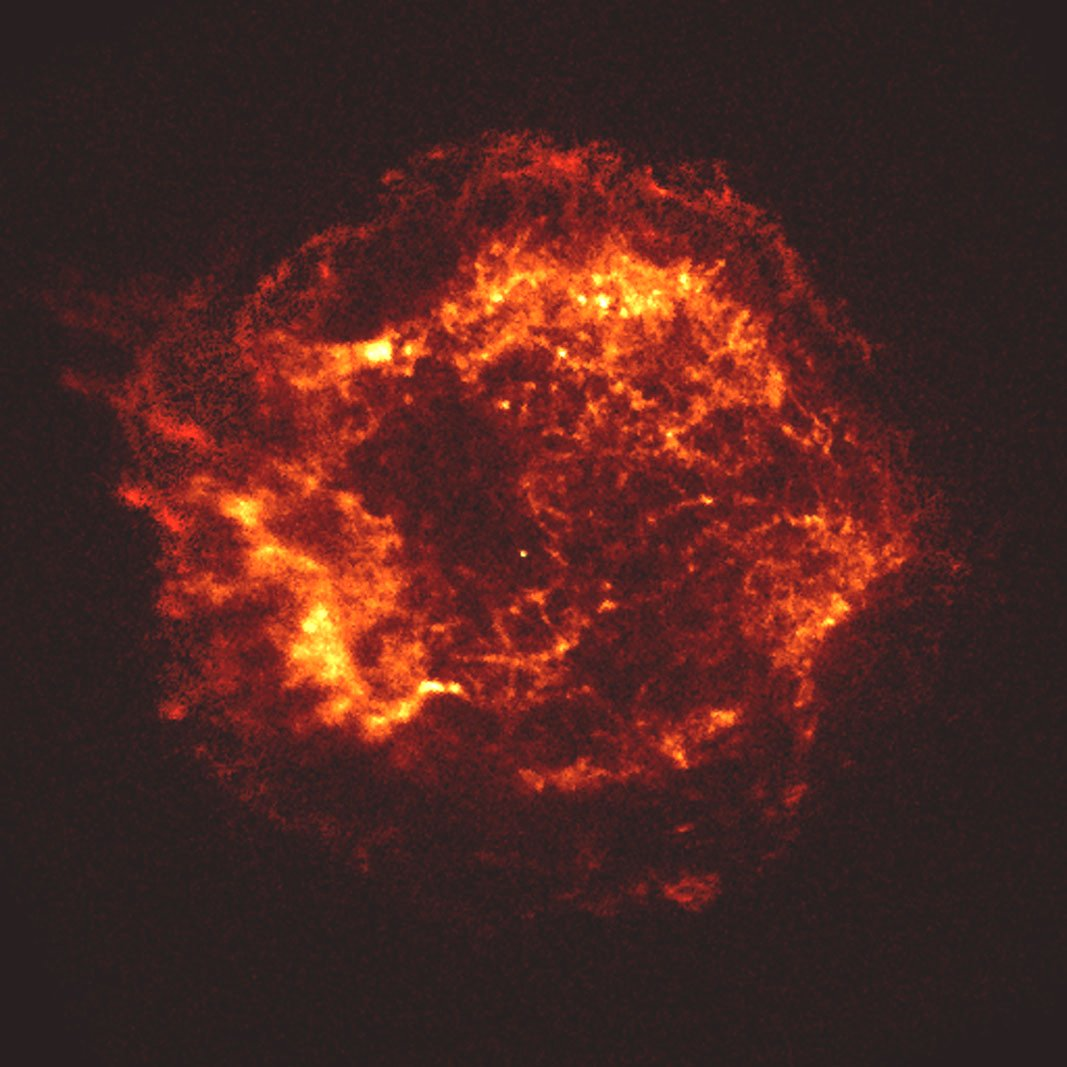
\includegraphics[keepaspectratio,height=15cm]{Cas_A}
\end{center}

\Tr
\twocolumn[\begin{center}{\blue Origin of cosmic rays}\end{center}]
%
\begin{itemize}
\item \colorbox{yellow}{Supernova blast waves}
\item[] Moving charge in static mag. field
\item[] Gyroradius $r=\frac{p}{ZeB} \quad (\vec{p} \perp \vec{B})$
\item[] $\rightarrow
         {\blue \left(\frac{p}{1~\rm{eV}}\right)=0.03 \cdot Z \left(\frac{B}{1~\mu\rm{G}}\right)
         \left(\frac{r}{1~\rm{m}}\right)}$
\item[] Shock wave~: extra factor $(\Gamma\beta)_{shock}$
\item Accelerator of size $R$
\item[] $r > R \rightarrow \text{particles~escape} \rightarrow E_{max}$
\item[] Typical~: $B \approx \mu\text{G} \quad R \approx \text{pc}$
\item[] $\rightarrow$ \colorbox{yellow}{Protons~: $E_{max} \approx 10^{15}$ eV}
\item[$\ast$] At a certain $r \rightarrow {\blue E_{Z}=Z E_{proton}}$
\item[$\ast$] $E>10^{19}~\text{eV} \rightarrow r>R_{galaxy}$
\item[] $\Rightarrow$ Extra-galactic origin
\end{itemize}

\newpage
%
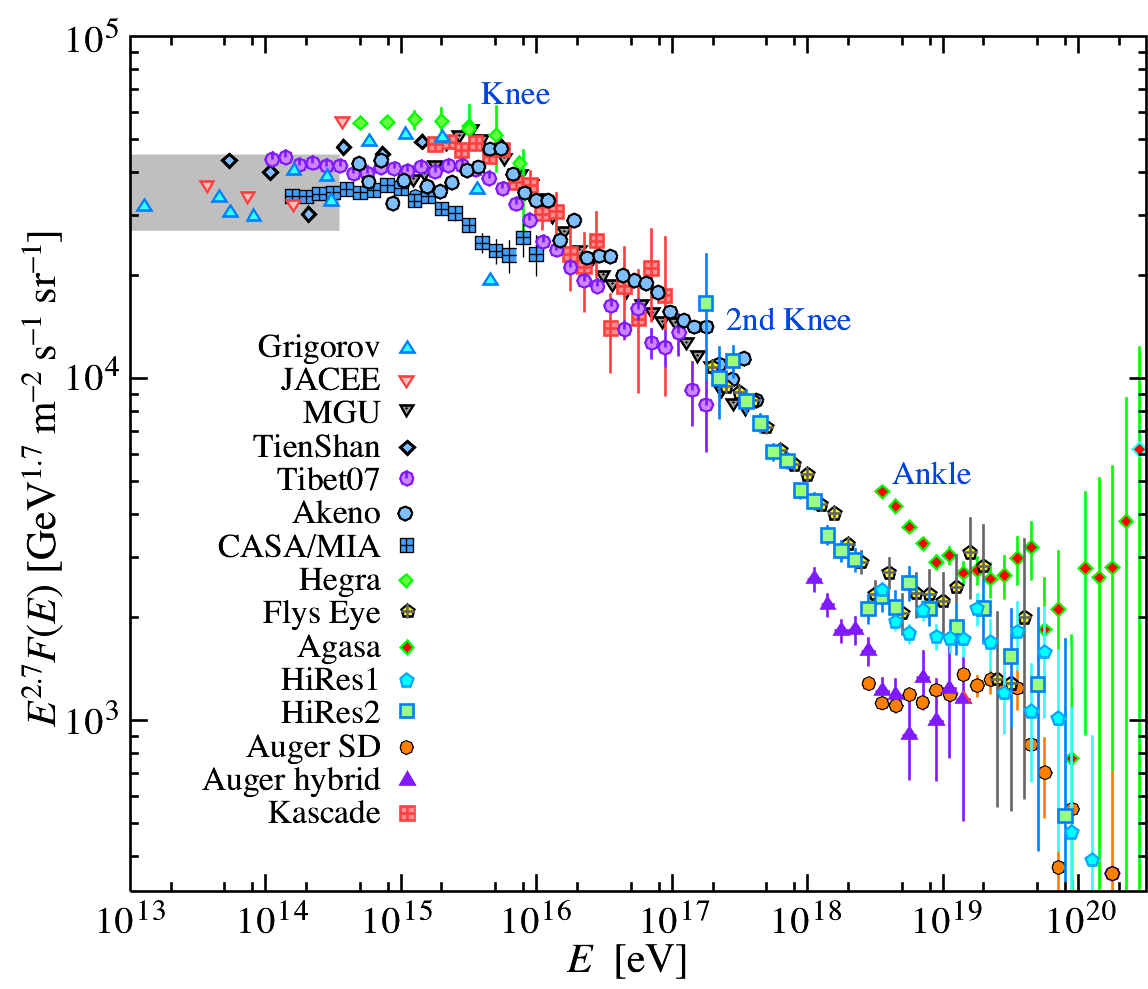
\includegraphics[keepaspectratio,width=10cm]{cr-all-scaled27}
%
\begin{itemize}
\item[] \colorbox{yellow}{What causes the slope change and 'ankle' ?}
\item[] Change in composition ?
\item[] Incorrect energy determination ?
\item[] New cosmic sources ?
\item[] \colorbox{yellow}{How can $E > 10^{20}$~eV exist ?} (GZK)
\end{itemize}

\Tr
\twocolumn[\begin{center}{\blue Analysis of cosmic ray cascades}\end{center}]
%
\begin{itemize}
\item Only sec. from atm. interactions observed
\begin{itemize}
\item[$\ast$] Properties of shower development
\end{itemize}
\item Multidim. $(N_{e},N_{\mu})$ shower analysis
\begin{enumerate}
\item At prim. vertex~: $\pi$, $K$, $\Lambda$, $\Xi$, $D$, ...
\item At shower maximum~: large $N_{e}$
\item After max.~: meson decays $\rightarrow \mu$, $\nu_{\mu}$
\item Even later~: $\mu$ decays $\rightarrow e$, $\nu_{e}$, $\nu_{\mu}$
\end{enumerate}
\item[] {\blue With increasing primary $E$}
\begin{itemize}
\item[$\ast$] Maximum closer to detector $(D_{max})$
\item[] $D_{max}$ from e.g. fluorescence meas.
\item[$\ast$] Larger sec. energies $\rightarrow$ longer lifetimes
\end{itemize}
\item[] {\blue $\rightarrow N_{e}/N_{\mu}$ increases}
\item[] $N_{e}/N_{\mu} \propto (E/A)^{\alpha} \quad (\alpha > 0)$
\end{itemize}

\newpage

\begin{itemize}
\item $A$ dependence (composition)
\item[] $N_{\mu} \propto (A/E)^{\alpha}\,N_{e}$
\item[] Certain prim. $E$ $\rightarrow N_{\mu} \propto A^{\alpha}\,N_{e}$
\begin{itemize}
\item[$\ast$] {\blue Heavy primaries $\rightarrow$ Muon rich showers}
\item[] Set scale limits by p and Fe
\item[$\ast$] {\blue $N_{e}/N_{\mu}$ (and $D_{max}$) $\rightarrow A \rightarrow E$}
\end{itemize}
\item[] \colorbox{yellow}{Quantitative analysis $\rightarrow$ MC needed}
\item Large discrepancies between various models
\item[] \colorbox{yellow}{Data needed to validate/tune models}
\item[$\ast$] CERN-LHC might provide insight here
\item[] {\blue Physics $E(Z)$ or cascade $E(A)$ effect~?}
\end{itemize}
